\chapter{System Implementation} \label{s-i}

\section{Introduction} \label{s-i--introduction}

This chapter described the high-level requirements and design of a system that blah blah blah.  The chapter started by describing blah.  The proposed solution was then discussed in section blah followed by blah in section blah, etc.
Blah blah is covered in further detail in Chapter 4 which describes the implementation of blah blah.

From design to implementation a few decisions and technologies changed.

Figure \ref{figure-application-stack-implementation}, shows the revised application stack for the implementation.

\begin{figure}[H]
  \centering
    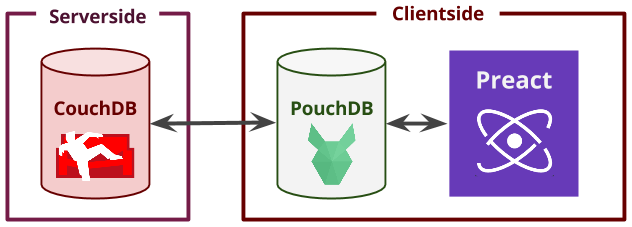
\includegraphics[width=\textwidth,height=\textheight,keepaspectratio]{application_stack_implementation}
  \caption{Overview of how the application stack is structured for the implementation}
  \label{figure-application-stack-implementation}
\end{figure}

The biggest change was the removal of Node.js stack including Express and Passport. As explained fully in section \ref{s-i--data-and-databases} the data manipulation and authentication functionality were handled through CouchDB.

\section{Packages} \label{s-i--packages}

During implementation and research into React and performance another framework was discovered called Preact. Preact, is a framework that attempts to recreate functionality of React but with the focus of performance. Using Preact means a better development experience. \cite{preact} Preact is 3kb in size in comparison to React which is 53kb in size.

The implementation therefor used Preact and was used for rendering views in the artefact.

One principle for software development is DRY (don't repeat yourself). One principle for software development is DRY (don't repeat yourself). ``Every piece of knowledge must have a single, unambiguous, authoritative representation within a system.'' \cite{DRY}

A good example of this is the `moment.js' package used in this artefact, this package handles most date and time related problems. To implement these features is not inherently difficult, but packages such as moment.js offer DRY tried and tested solutions. \cite{moment.js}

\section{Data and Databases} \label{s-i--data-and-databases}

As previously mentioned CouchDB is excellent at master-to-master replication of databases. This means syncing is easily implemented.

\colorbox{pink}{TODO: add diagram here}

The remote database and the local databases sync any changes between themselves, when the local database changes the recipes and brews in state are updated.

In the artefact design data section \ref{a-d--data} and following the decision was to use Node for a Express to handle data coming from the database and Passport to handle user authentication. However through the use of CouchDB and PouchDB it was found that there was no need for either of these technologies.

CouchDB has a user authentication system for handling permission and roles to documents. By default everyone is an admin in what they describe as the `admin party', this is recommended to be disabled but aids development with low barrier to entry when starting a new project.

As the data defines a lot of the structure of the application this authentication system has been leveraged for user authentication for the application.

\section{Interesting Problems} \label{s-i--interesting-problems}

During the implementation of this project several issues came up. This section discusses some of these issues.

Using newer technologies such as Webpack, ESLint, Babel and Preact come with difficulties. There is a generally a lack of support found online and even some issues can be so new they haven't been documented yet.

For example, with Preact during implementation there was an issue with a feature from React not being supported. This was short-circuit boolean templating, the author then reported this bug which was then fixed. Here having the Preact project as an Open Source project meant this could be fixed not just for this artefact but future users of Preact.

% describe this better with soundcloud example, also the virtual list thing

While testing the service worker code and implementation difficulties arise when caching files. Originally the author was manually unregistering the service worker then closing and reopening the tab.

Simply refreshing does not give you any updated version of the service worker files, this is due to the browser making the new page request before unloading the current page so the activated service worker is never released. \cite{refresh_sw}

As shown in figure \ref{figure-force-update-service-worker}, to solve this problem there is a `Force update on page load' option in the Chrome development tools.

\begin{figure}[H]
  \centering
    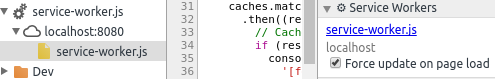
\includegraphics[width=\textwidth,height=\textheight,keepaspectratio]{force_update_service_worker}
  \caption{The `force update on page load' option}
  \label{figure-force-update-service-worker}
\end{figure}

One issue with frameworks and libraries expressed in section \ref{l-r--frameworks} was the lack of control of final code. Having to depend on the Brauhaus package due to a lack of home-brewing knowledge resulted in having to implement more of the library than potentially needed and ultimately a bigger file size reducing performance.

Keeping dependencies up to date is important mostly for security (see Snyk mentioned in section \ref{s-i--testing-summary}), a tool called Greenkeeper (shown in figure \ref{figure-greenkeeper}) was used through-out which monitors the project's dependencies and sends a Pull Request to the GitHub repository with an updated version of packages. This is great as these Pull Requests can be run through the continuous integration and if it passes the build can be merged straight away. \cite{greenkeeper}

\begin{figure}[H]
  \centering
    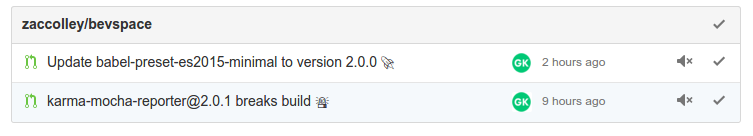
\includegraphics[width=\textwidth,height=\textheight,keepaspectratio]{greenkeeper}
  \caption{Example of Greenkeeper testing different package updates}
  \label{figure-greenkeeper}
\end{figure}

One problem when developing with service workers (and other web APIs) is needed SSL or https when in production. Thankfully, \verb|localhost| is ignored so these features can be used in development easily. Also with projects such as Let's Encrypt, adding SSL to a web site is free and easy. \cite{letsencrypt}

\section{Summary} \label{s-i--summary}

This chapter described the implementation of blah blah, which was based on the design described in Chapter 3. The implementation was introduced in section x and blah blah blah. Once the general implementation details had been introduced, several interesting implementation problems were addressed in section q, including the detailed coverage of blah blah.

\section{Testing and Evaluation} \label{s-i--testing-and-evaluation}

\subsection{Introduction} \label{s-i--t-a-e--i}

Chapters 3 and 4 described the design and implementation of blah blah, a system that blah blah blah.  In this chapter, we present a testing method and its results that show blah blah blah.  The chapter is organised as follows:  Section x introduces blah and describes blah.  Next, section y presents blah, etc.
The results of the tests are summarised in section z, before the solution is evaluated in section qqq.
Write what you did, why you did it and how you did it here.

\subsection{Testing Summary} \label{s-i--testing-summary}

The testing framework used was mocha and complemented by the `chai' and `sinon' packages. This meant simple and targeted tests could be created. \cite{mocha}

Using a headless browser such as PhantomJS means tests can be run automatically in a browser environment without having to open a browser such as Chrome or FireFox. \cite{phantomjs}

Now to run the tests created with mocha in PhantomJS a test runner called Karma was used. \cite{karma} This also handled processing the files through the same Webpack config that is used to build the site normally.

The tests created are for testing basic rendering of the Preact components and also that certain elements do not render if not authenticated. Figure \ref{figure-tests} shows tests running in a terminal environment.

\begin{figure}[H]
  \centering
    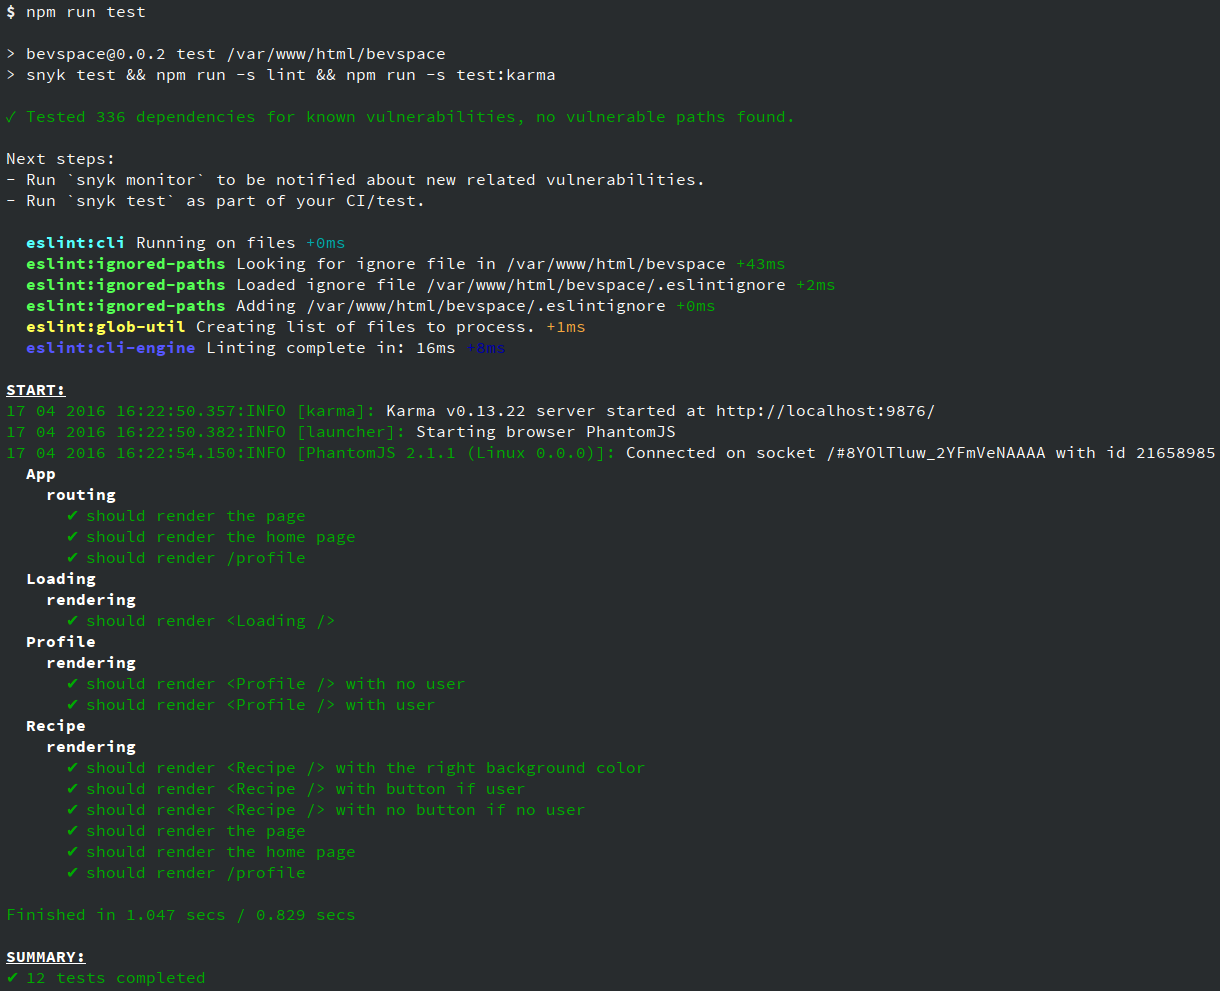
\includegraphics[width=\textwidth,height=\textheight,keepaspectratio]{tests}
  \caption{Output to the terminal when running `npm run test'}
  \label{figure-tests}
\end{figure}

(Note if ESLint passes linting, it usually doesn't output anything but for this screenshot the \verb|--debug| flag has been added)

For the continuous integration, the tests running include Snyk, linting and the previously mentioned rendering tests. \ref{a-d--continuous-integration}

\section{Evaluation} \label{s-i--evaluation}

Chapter 1 highlighted the problem of blah blah blah. Chapter 2 reviewed the state-of-the-art in blah and blah.  Chapter 3 identified a set of technical requirements underpinning the development of blah, and the implementation of a blah blah was described in Chapter 4.

The testing described in section x demonstrates that blah blah blah. In this section therefore, we evaluate the implementation and discuss issues in the underlying technologies that the implementation has highlighted.

The project since the project initiation document has changed dramatically. Due to the initial client moving away from the project a movement away from the home-brewing focus to the performance focus made sense. % add ref to appendix

Overall, where the project is weakened is through the planning and structuring. With more discipline this project could have been

Saying this, a lot of the technologies used in the project are in their infancy, as seen in section \ref{s-i--interesting-problems}. This means potentially the work flow, tools and technologies will all be outdated soon.

People and their needs don't change so much. Performance will always be important. So the research and work done in this area was very beneficial.

user testing should have been done

\subsection{Requirements Review} \label{s-i--requirements-review}

% This section reviews the implemented platform, referring back to the requirements to identify the extent to which each has been fulfilled, and reflecting on their relevance for future work. Each of the requirements is reintroduced and discussed in turn.

\subsubsection{Functional Requirements} \label{s-i--requirements--functional}

\subsubsection{Non-Functional Requirements} \label{s-i--requirements--non-functional}

The artefact should:

\begin{itemize}
  \item \textbf{Follow accessibility guidelines to ensure usage for those of hard of sight}

    When looking at the example of the items on the page, there was some need to improve the contrast.

    Fortunately using SASS (as chosen in section \ref{a-d--t--styling}) this is achieved very easily by changing \verb|color: \$brown;| producing \verb|\#943938| to \verb|color: darken(\$brown, 10\%);| producing \verb|\#6F2B2A|.

    Table \ref{table-contrast-changes} shows how the new darkened version of the brown colour is WCAG 2 AAA compliant.

    \begin{table}[H]
    \centering
    \begin{tabular}{|l|l|l|l|}
    \hline
    \textbf{Colour} & \textbf{Contrast Ratio} & \textbf{WCAG 2 AA Compliant} & \textbf{WCAG 2 AAA Compliant} \\ \hline
    \cellcolor[HTML]{943938}{\textbf{\textcolor{white}{\#943938}}} & 6.24 & Yes & No \\ \hline
    \cellcolor[HTML]{6F2B2A}{\textbf{\textcolor{white}{\#6F2B2A}}} & 8.81 & Yes & Yes \\ \hline
    \caption{Showing the compliance of the different colours against the background}
    \label{table-contrast-changes}
    \end{tabular}
    \end{table}

  \item \textbf{Be documented so that others can maintain}

    For future maintaining of the project documentation should be used. The README file shows instructions to build and work with the project. Comments through out components give explanation for code that isn't straight forward.

    A package called commitizen was used to enforce the contributing guidelines for project. \cite{commitizen}

  \item \textbf{Conform to the performance budget that is set in initial development}

    From the budget set in section \ref{table-performance-budget}, here are the results with the implemented site show in table \ref{table-performance-budget-results}.

    Notice how times change before and after caching with the service worker.

    \begin{table}[H]
    \centering
    \begin{tabular}{|l|l|l|l|}
    \hline
    \textbf{Site}     & \textbf{Start Render} & \textbf{Document Complete} & \textbf{Fully Loaded} \\ \hline
    Malt.to           & 2.190s                & 3.998s                     & 4.145s                \\ \hline
    Proposed solution & 1.752s                & 3.198s                     & 3.316s                \\ \hline
    Implementation & 0.000s                & 0.000s                     & 0.000s                \\ \hline
    Implementation w/ SW & 0.000s                & 0.000s                     & 0.000s                \\ \hline
    \end{tabular}
    \caption{Performance budget calculation with results}
    \label{table-performance-budget-results}
    \end{table}

  \item \textbf{Pass tests generated throughout and running through continuous integration (such as Travis CI)}

    As described in detail in section \ref{s-i--testing-summary}, the artefact is passing all tests including Snyk, Linting and Karma. However, by the nature of Snyk looking for vulnerabilities constantly without maintenance these tests could fail.

\end{itemize}

\section{Testing and Evaluation Summary} \label{s-i--testing-and-evaluation-summary}

This chapter introduced blah and blah.  In section x a series of tests were described which demonstrated blah blah.
An evaluation of blah blah was then presented in section y.  Section z revisited the requirements described in Chapter 3 and identified that blah blah blah. Finally in section q the aspects of blah blah were discussed.
